\Chapter{}
\chapter{Metodología}
    \section{Área de estudio}
        La investigación se enfocó en imágenes Landsat MSS y TM de diversas regiones a nivel mundial. La Antártida se excluye por su homogeneidad espectral, dominada por extensas áreas de hielo y nieve, lo que dificulta la diferenciación de coberturas y complica la armonización satelital \autocite{kokhanovsky2019retrieval}. De manera similar, las regiones oceánicas se descartan debido a su uniformidad espectral, lo que limita la variabilidad en la reflectancia \autocite{estrella2021spectral}. Por lo tanto, el estudio se centra en áreas continentales no homogéneas en términos de reflectancia.
    \section{Diseño de investigación}
        \subsection{Tipo de investigación}
            Aplicada, ya que tiene como objetivo principal utilizar técnicas avanzadas de inteligencia artificial para mejorar la armonización de las imágenes Landsat MSS. La finalidad es proporcionar herramientas más eficientes y precisas para el monitoreo global, beneficiando a investigadores, entidades gubernamentales y organizaciones relacionadas con el estudio de la superficie terrestre.
        \subsection{Nivel de investigación}
            Descriptiva y exploratoria. Es descriptiva porque se analizarán las características y ventajas de las técnicas de aprendizaje profundo en la armonización de imágenes MSS. Es exploratoria, ya que se busca comprender y evaluar cómo estas técnicas pueden mejorar la calidad y precisión de estas imágenes, un área con desafíos y oportunidades para la innovación.
	\subsection{Enfoque}
            Cuantitativo. Se utilizarán herramientas y técnicas estadísticas para evaluar la eficacia de las técnicas de aprendizaje profundo en la armonización de las imágenes. Esto implica comparar imágenes antes y después de la armonización, evaluando la calidad de las imágenes resultantes y cotejándolas con métodos tradicionales. Los resultados se expresarán numéricamente, utilizando indicadores como porcentajes de mejora, errores cuadráticos medios, entre otros relevantes.

    \section{Población y muestra}
    
        \subsection{Población}
            La población objeto de este estudio consiste en la totalidad de las imágenes obtenidas por el sensor MSS del satélite Landsat que cubren las regiones continentales globales, excluyendo la Antártida y las regiones oceánicas, durante el período de tiempo comprendido entre 1982 y 1999. Estas imágenes están disponibles a través de las bases de datos de Landsat, las cuales proporcionan un registro histórico completo y accesible para la extracción de los datos necesarios para el presente estudio.

        \subsection{Muestra}
            El diseño de muestreo adoptado es de tipo probabilístico. Se seleccionarán unidades de muestreo de manera aleatoria, lo cual es esencial para garantizar la independencia estadística y la representatividad dentro del universo de las imágenes MSS de Landsat. De acuerdo con los principios establecidos por \textcite{hernandez2014recoleccion}, se ha determinado un tamaño de muestra representativo del conjunto total de la población.

            Para la implementación de técnicas de clasificación supervisada, tales como algoritmos de armonización basados en aprendizaje profundo, es imperativo contar con un conjunto de datos dividido en muestras de entrenamiento y validación. Siguiendo las recomendaciones de \textcite{belgiu2016random}, las muestras de entrenamiento deben ser: 1) estadísticamente independientes de las muestras de validación, 2) equilibradas en términos de distribución de clases, 3) representativas de las variabilidades espectrales objetivo, y 4) suficientemente amplias para cubrir la complejidad de los datos. Con base en estos criterios, para este estudio se destinará el 70\% de las imágenes seleccionadas aleatoriamente para el entrenamiento del modelo y el 30\% restante para la validación del mismo \autocite{nami2018spatial}. La asignación de las imágenes a cada uno de estos conjuntos se realizará mediante un algoritmo de selección aleatoria que asegure la aleatoriedad de la división \autocite{gigovic2019testing}.
        
    \section{Procedimiento, técnicas e instrumentos de recolección de información}

       \subsection{Obtención de Datos de Entrada}
            \subsubsection{Selección por localización}
                Para garantizar la eficacia y precisión de la investigación, se llevó a cabo una meticulosa selección de imágenes para el estudio. A continuación, se detalla el procedimiento de selección:
                
                \begin{enumerate}
                    \item Como punto de partida, se generaron puntos de manera aleatoria alrededor del mundo, resultando en un total inicial de 10 000 puntos. Estos puntos sirvieron como centroides para definir buffers cuadrados con dimensiones de 30 720 metros por lado.
                    
                    \begin{figure}[H] 
                        \caption{\doublespacing \\ \textit{Generación de 10 000 puntos aleatorios a nivel mundial.}} 
                        \centering
                        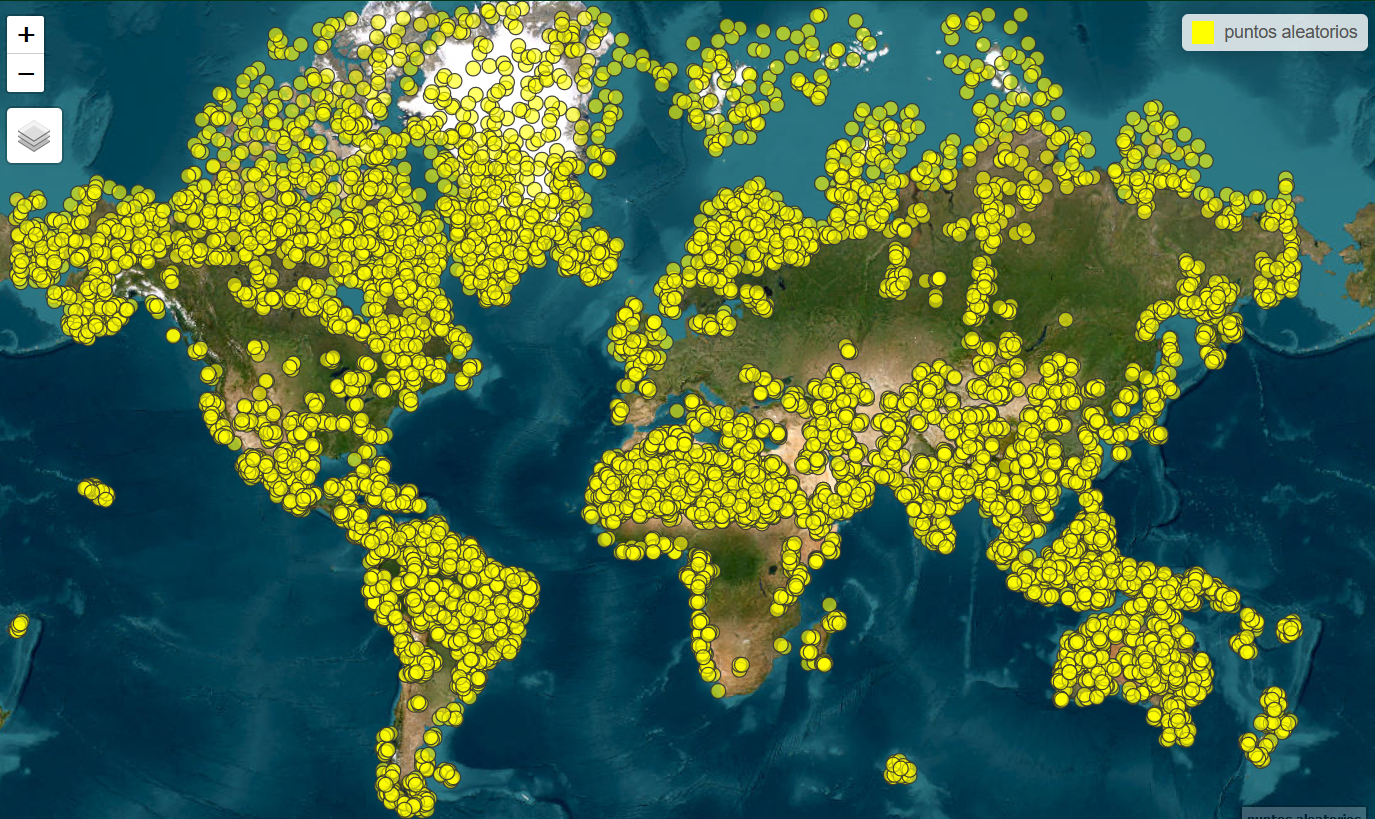
\includegraphics[width=0.7\linewidth]{2_CAPITULO0/IMG/1000points.png}
                        \begin{justify}
                            \textit{Nota.} Los puntos no excedieron los límites del WRS-2 (desde Landsat 4 hasta Landsat 9), que corresponden a las áreas o segmentos de captura de todas las imágenes Landsat, incluyendo los sensores más recientes.
                        \end{justify}                    
                        \label{1000points}
                    \end{figure}

        
                    \item Con los puntos geográficos establecidos, se procedió a seleccionar imágenes específicas. Se optó por imágenes MSS pertenecientes exclusivamente a las misiones Landsat 4 y 5, ya que coinciden con las imágenes obtenidas por el sensor TM de las mismas misiones durante el período de 1982 a 1999.
                
                    \item Una condición crucial en esta fase fue asegurar que el área definida por cada buffer estuviera íntegramente contenida dentro de al menos una imagen MSS y una imagen TM. Este criterio busca prevenir truncamientos o limitaciones en la amplitud de las imágenes.
                    
                    \item Se excluyeron ciertas áreas geográficas del proceso: específicamente, regiones de la Antártida y zonas mayormente oceánicas, para asegurar la relevancia y calidad del conjunto de datos final.
                    
                    \item Tras aplicar todos los criterios anteriores, de los 10 000 puntos iniciales, solo 8 546 satisfacían todas las condiciones y, por lo tanto, fueron retenidos para el estudio.
                \end{enumerate}
            \subsubsection{Selección por Tiempo y Calidad}
                Tras el filtro geográfico inicial, se procedió a una selección más detallada basada en criterios temporales y de calidad. A continuación se describe el procedimiento adoptado:
                
                \begin{enumerate}
                    \item De los 10 000 puntos iniciales, solo 8 546 cumplían con los criterios de localización. Para estos puntos seleccionados, se llevó a cabo una comparación temporal entre las imágenes de los sensores MSS y TM.
                
                    \item La condición impuesta fue que las imágenes de ambos sensores debían tener un diferencial temporal no superior a 10 minutos. Es decir, por cada punto, se retuvieron solo aquellos pares de imágenes MSS y TM que hubieran sido capturadas en un intervalo de tiempo menor o igual a 10 minutos entre ellas.
                    
                    \item Es importante mencionar que este filtro temporal se aplicó considerando imágenes de los niveles Tier 1 y Tier 2 para ambos sensores. Debido a este riguroso criterio, no todos los puntos conservaron la misma cantidad de imágenes, y algunos incluso quedaron sin imágenes que cumplieran con este requisito.
                    
                    \item Posterior al filtro temporal, se implementó un filtro de calidad basado en la nubosidad. Se utilizó la banda de calidad (QA), específicamente de las imágenes del sensor TM, para evaluar la presencia de nubes o sombras. El criterio adoptado fue que las imágenes retenidas no debieran tener una cobertura de nubes o sombras que superara el 15\% del área del buffer generado por el punto dentro de la extensión de la imagen.
                    
                    \item Al concluir estos filtros, se obtuvo un conjunto final de imágenes (15 882 pares) obtenidos de 5 877 puntos filtrados de  que satisfacen tanto los criterios de diferencial temporal como los de calidad en relación con la nubosidad.
                \end{enumerate}
                
                Este enfoque garantizó un conjunto de datos con alta precisión temporal y calidad visual, minimizando las distorsiones o interferencias potenciales debido a la nubosidad.

        \subsection{Corrección Geométrica de las Imágenes MSS}

            El propósito de este proceso es asegurar una alineación precisa entre las imágenes MSS y TM. A continuación, se detallan las etapas de la corrección geométrica:
            
            \subsubsection{Lectura y Preprocesamiento de Imágenes}
                Se cargan las imágenes MSS y TM, y son normalizadas para tener valores reales de reflectancia. Se seleccionan únicamente las bandas que coinciden entre las imágenes, garantizando su comparabilidad.
            
            \subsubsection{Extracción y Coincidencia de Características}
                Con la ayuda de modelos de aprendizaje profundo como LightGlue, se identifican puntos clave en ambas imágenes. Estos puntos son luego emparejados para determinar la desalineación entre las imágenes MSS y TM.
                
                \begin{figure}[H] 
                    \caption{\doublespacing \\ \textit{LightGlue: Emparejamiento de Características en Imágenes con Mecanismo Adaptativo.}} 
                    \centering
                    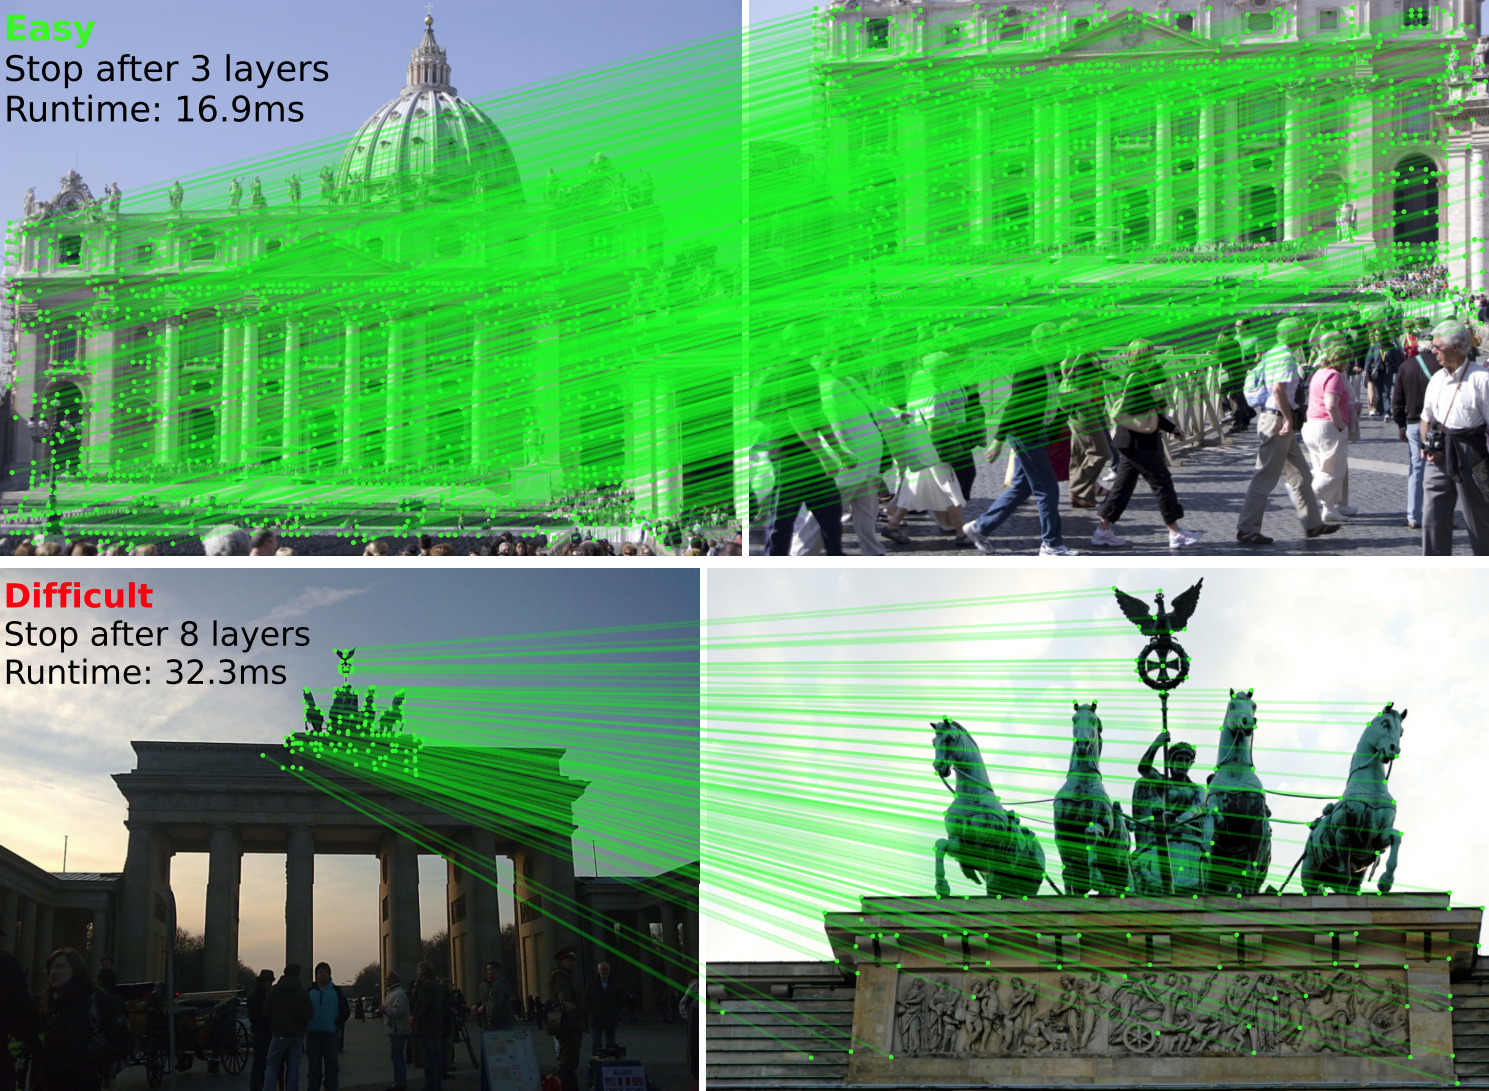
\includegraphics[width=0.7\linewidth]{2_CAPITULO0/IMG/cvg.png}
                    \begin{justify}
                        \textit{Nota.} La interfaz de 'LightGlue' exhibe dos ejemplos: uno 'fácil' con características emparejadas del Vaticano en 16.9ms y tres capas de procesamiento, y otro "difícil" de un monumento con estatuas, procesado en 32.3ms y ocho capas. Obtenido de \textcite{LightGlue2023}.
                    \end{justify}                    
                    \label{cvg}
                \end{figure}
                
               
            \subsubsection{Determinación del Desplazamiento Espacial}
                Usando los puntos clave coincidentes, se estima el desplazamiento espacial entre las imágenes. Este desplazamiento señala cuánto y cómo se desalinean las imágenes en términos de píxeles.

                \begin{figure}[H] 
                    \caption{\doublespacing \\ \textit{Emparejamiento Adaptativo de Características con LightGlue: De Alta Resolución (HR) a Baja Resolución (LR).}} 
                    \centering
                    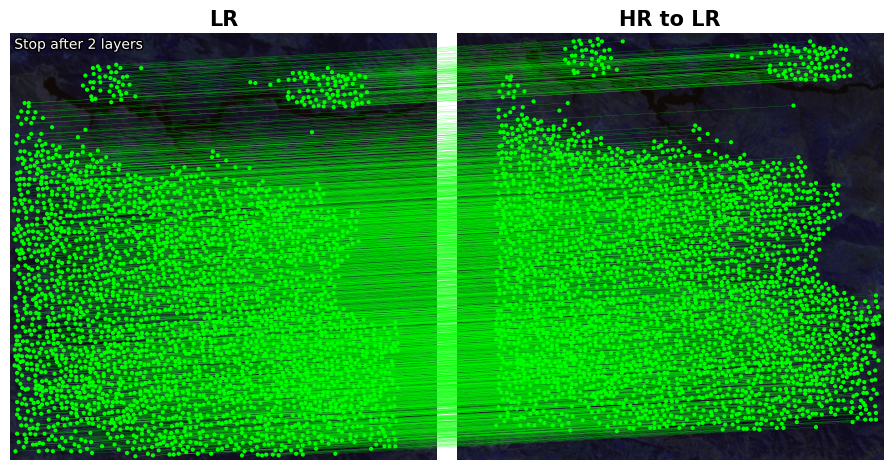
\includegraphics[width=0.8\linewidth]{2_CAPITULO0/IMG/hr_to_lr.png}
                    \begin{justify}
                        \textit{Nota.} Se observan superposiciones verdes de características detectadas, deteniéndose en ambas tras dos capas, evidenciando la eficacia de "LightGlue".
                    \end{justify}                    
                    \label{hr_to_lr}
                \end{figure}
                
            \subsubsection{Refinamiento Subpíxel y Convolución en 2D}
                Para refinar la corrección, se recurre a la transformada de Fourier. Esta técnica, mediante la función de correlación cruzada en el dominio de frecuencia, equivale a una convolución en 2D en el dominio espacial. La convolución en 2D es una operación que toma dos imágenes de entrada y produce una tercera imagen como salida, siendo una técnica fundamental en procesamiento de imágenes para filtrar y enfocar. Aquí, ayuda a identificar desplazamientos subpíxeles basados en el contenido de frecuencia de las imágenes.
                
                \begin{equation}
                    X(f) = \int_{-\infty}^{\infty} x(t) \cdot e^{-j2\pi ft} dt
                \end{equation}
            
                Donde \(X(f)\) es la transformada de Fourier de la señal \(x(t)\).
                
                
                Con base en el desplazamiento determinado y su refinamiento subpíxel, las imágenes MSS son alineadas geométricamente con las TM.
                
                Las imágenes MSS corregidas se presentan junto con las TM para confirmar visualmente la alineación. A través del proceso de corrección, se observa una mejora notable en la alineación, evidenciada por la reducción del desajuste visual entre las imágenes. Esta mejora se logra mediante correcciones tanto a nivel de píxel como subpíxel, lo que resulta en una superposición más precisa entre las imágenes MSS y TM.
                
                \begin{figure}[H] 
                    \caption{\doublespacing \\ \textit{Comparativa de Alineación: Imágenes MSS, TM y MSS Corregida.}} 
                    \centering
                    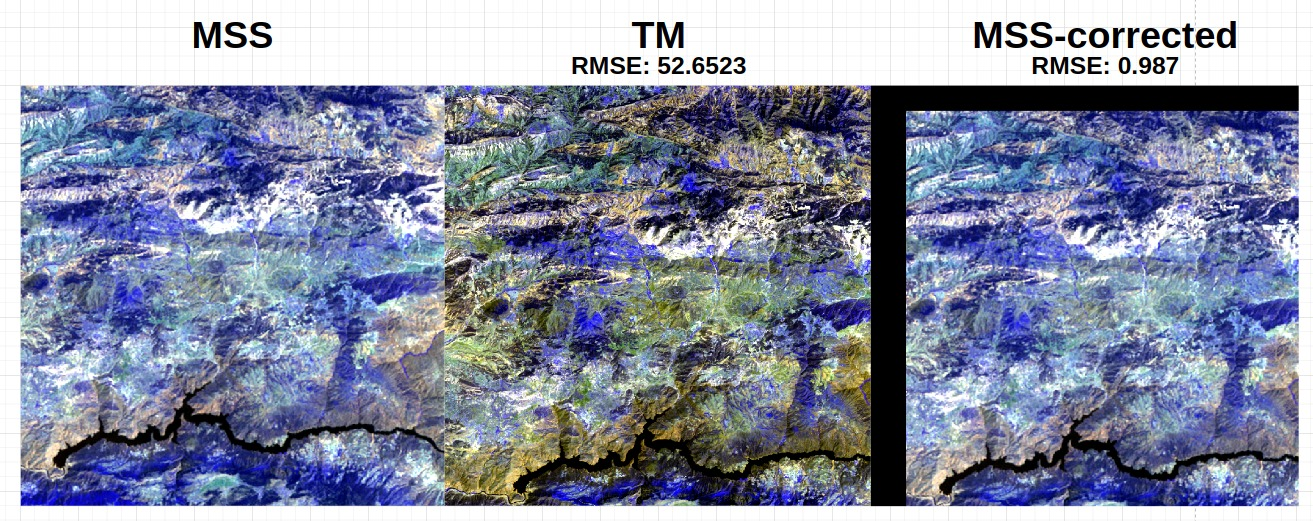
\includegraphics[width=0.8\linewidth]{2_CAPITULO0/IMG/tm_mss_rmse.png}
                    \begin{justify}
                        \textit{Nota.} El contraste entre la imagen MSS original y la corregida resalta con una reducción significativa del error RMSE de 52.6523 a 0.987, evidenciando la eficacia de las correcciones a nivel de píxel y subpíxel para lograr una alineación casi perfecta.
                    \end{justify}                    
                    \label{tm_mss_rmse}
                \end{figure}
                
        \subsection{Desarrollo del Modelo MSS2TM para Alineación Espacial y Espectral}
            Para lograr una coherencia óptima entre las imágenes MSS y TM, es fundamental establecer una correspondencia tanto espacial como espectral entre ellas. El objetivo es convertir las imágenes MSS para que sean similares en resolución y calidad a las imágenes TM. Para ello, desarrollamos el modelo de aprendizaje profundo llamado MSS2TM. 
            
            MSS2TM es entrenado utilizando pares de imágenes MSS y TM que comparten características espectrales similares. Al entrenar el modelo con estas imágenes, MSS2TM aprende a mapear y transformar las características de las imágenes MSS de manera que se alineen con las de las imágenes TM. En términos prácticos, esto significa que las imágenes MSS procesadas por este modelo tendrán una calidad y resolución similar a las TM en las bandas que ambas comparten.
            
            Este proceso no solo mejora la resolución espacial de las imágenes MSS, sino que también ajusta sus valores espectrales, lo que permite una comparación más directa y precisa entre las dos imágenes.
                
        \subsection{Generación de Bandas Virtuales en Imágenes MSS}
            Una vez que las imágenes MSS se alinean espectral y espacialmente con las TM gracias al modelo MSS2TM, el siguiente paso es generar bandas sintéticas o virtuales para las MSS que existen en las TM pero no en las MSS. 
            
            Para lograr esto, se implementa una técnica de aprendizaje profundo que utiliza las bandas armonizadas previamente como entradas y busca generar bandas faltantes como la banda azul y la banda SWIR. El modelo se entrena utilizando las bandas coincidentes de las imágenes MSS armonizadas como características de entrada y las bandas objetivo de las imágenes TM como salida esperada. 
            
            Esta técnica de generación de bandas virtuales no solo permite ampliar la información espectral de las imágenes MSS, sino que también garantiza que esta información sea coherente y comparable con las imágenes TM originales. Esta coherencia es esencial para garantizar que cualquier análisis posterior que se realice utilizando estas imágenes sea preciso y confiable.
                
        

            \begin{figure}[H] 
                \caption{\doublespacing \\ \textit{Modelo de armonización para imágenes Landsat MSS.}} 
                \centering
                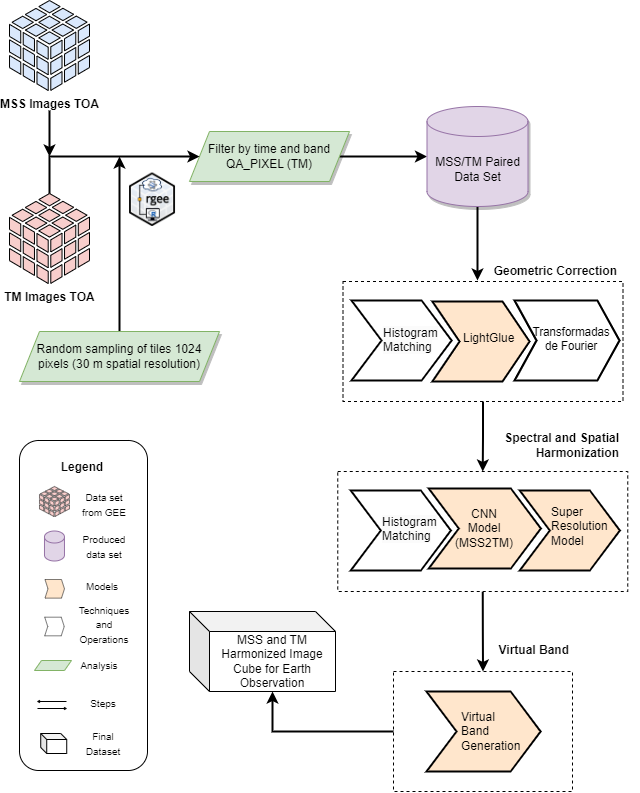
\includegraphics[width=0.95\linewidth]{2_CAPITULO0/IMG/modelo.png}
                \begin{justify}
                    \textit{Nota.} El esquema presenta una metodología de armonización de imágenes de sensores MSS y TM: comienza con imágenes TOA, sigue con correcciones geométricas y transformadas de Fourier via LightGlue, continúa con armonización espectral y espacial mediante modelos CNN y culmina con un cubo de imagen armonizado para la creación de bandas virtuales.
                \end{justify}                    
                \label{modelo}
            \end{figure}

    \section{Análisis estadístico}
        En la fase de preparación para la validación de los modelos desarrollados, se diseñó un enfoque de análisis estadístico detallado. Este diseño metodológico fue crucial para asegurar que, una vez aplicados, los modelos pudieran demostrar un ajuste adecuado a los datos de entrenamiento y una generalización efectiva a nuevos conjuntos de datos.
        
        Se decidió que el RMSE se calcularía para estimar la discrepancia entre las predicciones de los modelos y los valores observados, buscando valores bajos como indicativos de precisión. Además, se preveía el uso del coeficiente de correlación de Pearson para examinar la relación lineal entre las predicciones y los valores reales.
        
        Para evaluar la calidad de las imágenes producidas por los modelos, se eligió el Índice de Similitud Estructural (SSIM). Un valor alto en esta métrica indicaría una similitud estructural satisfactoria con las imágenes de referencia.
        
        Se estableció que se realizaría un análisis visual preliminar de las salidas de los modelos, con el fin de detectar desviaciones preliminares o inconsistencias potenciales. Para la selección de variables significativas en los modelos, se planificó utilizar un valor-p menor a 0.05 y un coeficiente R² mayor a 0.75 como umbrales para su inclusión.